\documentclass{udpreport}
\title{Creación de paquetes utilizando Scapy y validación con Wireshark}
\author{Integrantes: Thomas Muñoz, Ignacio Yanjari, Dagoberto Navarrete, Ignacio López.}
\date{Marzo de 2016}
\usepackage{graphicx}
\graphicspath{ {img/} }
\udpschool{Escuela de Informática y Telecomunicaciones}

\begin{document}
\maketitle
\tableofcontents
\chapter{Actividades}
	\section{Instalacion de software}

	\section{Creacion de Paquetes}
		
	\section{Cuestionario}
	
	  1.-¿Qué pasa cuando envío un paquete a la dirección FF:FF:FF:FF:FF:FF? ¿Quienes
	     lo reciben? ¿Por qué?\\
	     
	     Cuando enviamos un paquete a la dirección FF:FF:FF:FF:FF:FF, este fue enviado a todos los equipos dentro de la red
 +	     Ethernet. Esto es debido a que la dirección antes mencionada esta designada para que la difusión de nuestro paquete sea
 +	     enviado a cada dispositivo conectado a nuestra red LAN, a este tipo de difusión se le conoce como “Broadcast”.\\
 
  	  2.-¿Qué pasa cuando envío un paquete a una MAC de otro equipo? ¿Quienes lo
  	      pueden recibir? ¿Por qué?\\
 -	      
 +	      Cuando enviamos un paquete a la dirección MAC de otro equipo dentro de la red Ethernet, solamente el equipo que poseía
 +	      esa dirección fue capaz de recibirlo. Esto ocurre puesto a que, como indicamos anteriormente, al paquete le dimos una
 +	      MAC de destino fija, entonces el paquete se encargó de viajar solamente al equipo que poseía esa dirección\\
 
  	  3.-¿Qué sucede si envía un paquete a una MAC que no corresponda a ningún equipo
  	      de la red? ¿Quienes lo pueden recepcionar? ¿Por qué?\\
 -	      \begin{figure}[h]
    			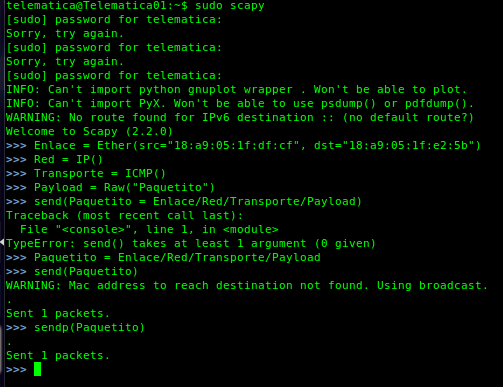
\includegraphics[width=4cm, height=4.3cm]{MAC_noconocida.png}
 +	      Cuando enviamos un paquete a una dirección MAC que no correspondía a ningún equipo de la red, al enviarlo nos apareció
 +	      el mensaje: “WARNING: Mac address to reach destination not found. Using Broadcast.” Y posteriormente el paquete fue
 +	      enviado a todos los equipos pertenecientes a la red Ethernet.Este usa el broadcast para asi poder tener todas sus MAC y       dejarlas asi mismo registradas en una lista llamada arp. En la cual luego de lograr esto revisa si la MAC de destino          existe o no,como este caso se trata de una MAC que no corresponde a la red responde con un WARNING\\

 +	     
	      

\chapter{Conclusión}
  
\begin{thebibliography}{x}

\end{thebibliography}
\end{document}
